% chktex-file 12
% chktex-file 44

\documentclass{article}
\usepackage{amsmath}
\usepackage{amssymb}
\usepackage{tabularx}
\usepackage{bm}
\usepackage{graphicx}
\usepackage[a4paper, top=0.75in, bottom=0.75in]{geometry}

\graphicspath{{./images/}}

\title{Clustering}
\author{David Robinson}
\date{}
\setlength{\parindent}{0pt}

\begin{document}

\maketitle

\textbf{Clustering} is an unsupervised learning technique used to group similar data points together based on specific criteria. The objective is to maximize similarity within a cluster and minimize similarity between clusters.

\subsection*{Types of Clustering}
\begin{itemize}
    \item \textbf{Hierarchical Clustering}: Builds a hierarchy of clusters.
    \item \textbf{K-Means Clustering}: Partitions data into a predefined number of clusters.
    \item \textbf{Density-based Clustering (DBSCAN)}: Clusters points based on density and handles outliers well.
\end{itemize}

\section*{Hierarchical Clustering}

Hierarchical algorithms create a hierarchical decomposition of objects based on similarity. The hierarchical decomposition is represented with a \textbf{dendrogram}, which is a tree-like diagram where height measures how similar the data points are.

\begin{center}
    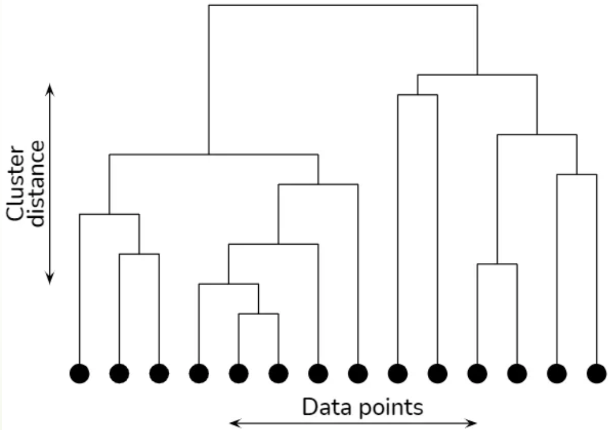
\includegraphics[scale=0.5]{dendrogram.png}
\end{center}

\subsection*{Bottom-Up (Agglomerative) Approach}
\begin{enumerate}
    \item Each data point is first treated as its own cluster.
    \item At each step, the closest clusters are merged based on a distance metric.
    \item The process continues until all data points are merged into a single cluster.
\end{enumerate}

\subsection*{Top-Down (Divisive) Approach}
\begin{enumerate}
    \item The dataset starts a single cluster.
    \item At each step, K-Means is applied to split clusters.
    \item The process continues until each data point is in its own cluster.
\end{enumerate}

\section*{K-Means Clustering}

K-Means clustering minimizes the Euclidean distance between points and their respective cluster centroids. The cluster quality is measured with a sum of the distances from each point to the cluster centroid.

\subsection*{Algorithm}

\begin{enumerate}
    \item Choose the number of clusters $K$.
    \item Initialize $K$ cluster centroids.
    \item Assign each point to the nearest centroid.
    \item Update the centroids by averaging the points in each cluster.
    \item Repeat steps 3--4 until the centroids do not change or the amount of change falls below a threshold.
\end{enumerate}

\subsection*{Strengths}

\begin{itemize}
    \item $O(tKn)$ Time Complexity: K-Means has a time complexity of $O(tKn)$ where $n$ is the number of data points, $K$ is the number of clusters, and $t$ is the number of iterations. $K$ and $t$ are much smaller than $n$ so the runtime is relatively fast.
\end{itemize}

\subsection*{Limitations}

\begin{itemize}
    \item Relies on dataset mean: K-Means is only applicable when the mean of the data points can be calculated.
    \item Requires pre-determined $K$: The number of clusters must be specified at the beginning, which may not be easy to determine.
    \item Sensitive to noise and outliers: K-Means struggles with noisy data and outliers as it significantly affects the cluster centroids.
    \item Not suitable for non-convex clusters: K-Means assumes clusters are spherical.
\end{itemize}

\end{document}